\documentclass[10pt,a4paper]{amsart}

\usepackage{graphicx}

\author{Vaibhav Karve}
\title{Progress report on study of NYC traffic}

\begin{document}

\date{\today}
\maketitle

\section{Restricting to a block}
We restrict our attention to the block between W. 44th to 45th St. and
8th to 9th Ave. This block was selected at random. On extracting the
data from the data file for 2011, we see that these streets are all one-way
access only.

\subsection{Naming convention}
\subsubsection{Intersections}
	\begin{itemize}
		\item \(A=\) W. 44th St. and 8th Ave. (Node\_id = 42435671)
		\item \(B=\) W. 44th St. and 9th Ave. (Node\_id = 42443561)
		\item \(C=\) W. 45th St. and 8th Ave. (Node\_id = 42432700)
		\item \(D=\) W. 45th St. and 9th Ave. (Node\_id = 42432703)
	\end{itemize}

\subsubsection{Roads}
	\begin{itemize}
		\item \(BA\) (Link\_id = 128255)
		\item \(AC\) (Link\_id = 169017)
		\item \(CD\) (Link\_id = 182993)
		\item \(DB\) (Link\_id = 181188)
	\end{itemize}
		
We restrict our attention to only these links, one at a time. For each
link, from the database, we extract 2 separate arrays: one giving the
average travel time in seconds, for every hour of the year; and the other
giving the number of trips on that used that link, for every hour of the
year.

\subsection{Periodicity Analysis}
\subsubsection{Stratifying the data}
Intuitively, one may expect that traffic patterns repeat themselves
every \(7\) days (weekly) or maybe every \(30\) days (monthly). Or
perhaps, there is no such periodicity. Whatever be the case, the
periodicity should not be imposed, but rather should be inferred
from the data itself. To do so, we we assume a particular period in
days, call it \texttt{period} and divide the entire data into
\(24\times\mathtt{period}\) number of bins. This converts our data
from flat lists of trips and traveltimes to something that may be
viewed as stratified data. 

Stratified data now looks like:
	\[ \left( \begin{array}{ccccc}
	\mathbf{Stratum\_1} & \mathbf{Stratum\_2} & \mathbf{Stratum\_3} & \cdots &
		\mathbf{Stratum\_N} \\
	5 & 2 & 32 & \cdots & 10 \\
	? & 7 & 5 & \cdots & ? \\
	33 & ? & 12 & \cdots & ? \\
	\vdots & \vdots & \vdots & \cdots & \vdots
	\end{array} \right)\]

Here, \(N=24\times\mathtt{period}\). We let period range from \(2\)
to \(38\) for our periodicity analysis.

\subsubsection{Missing values}
The question marks (?) in the above matrix correspond to those hours for which
we have no data on our link. This ofcourse does not mean that there is no
traffic on that link at that time, just that we don't know what it it. These
are to be treated as missing values in our data and need to be somehow
inferred.

The links \(BA\), \(AC\), \(CD\) and \(DB\) have \(20\%\), \(0\%\), \(0\%\)
and \(1\%\) of their values missing, respectively.

The most natural first approximation for these missing values is the mean
value of the corresponding stratum to which each missing value belongs.

The Inferred Stratified data looks like:
	\[ \left( \begin{array}{ccccc}
	\mathbf{Stratum\_1} & \mathbf{Stratum\_2} & \mathbf{Stratum\_3} & \cdots &
		\mathbf{Stratum\_N} \\
	5 & 2 & 32 & \cdots & 10 \\
	Mean_1 & 7 & 5 & \cdots & Mean_N \\
	33 & Mean_2 & 12 & \cdots & Mean_N \\
	\vdots & \vdots & \vdots & \cdots & \vdots
	\end{array} \right)\]

Here, we calculated the mean for each stratum by ignoring the missing values.

\subsubsection{Stratified variances}
To establish the optimal choice of \texttt{period} for the data, we calculate
the variance of the inferred stratified data we obtained in the previous
subsection.
	\[\text{Variance of stratified data} \approx \frac{1}{n}
		\sum_n{\text{Variance of each stratum}}\]
where \(n=24\times\mathtt{period}\) is the total number of strata.

If there truly does exist a periodicity in the data, for the correct
\texttt{period}, the values within each stratum will lie close to each other
and hence, the variance will be minimized. Hence, we look for dips in the
variance.

\subsection{Conclusion of periodicity analysis}
We calculate the variance for each value of \texttt{period} from \(2\) to
\(38\). The graph of the variances for link \(BA\) for the No.\ of Trips
during 2011 is given below:

\begin{figure}[hbtp]
\centering
\caption{The dips in variance correspond to \(\mathtt{period}=7,14,21,35\).}
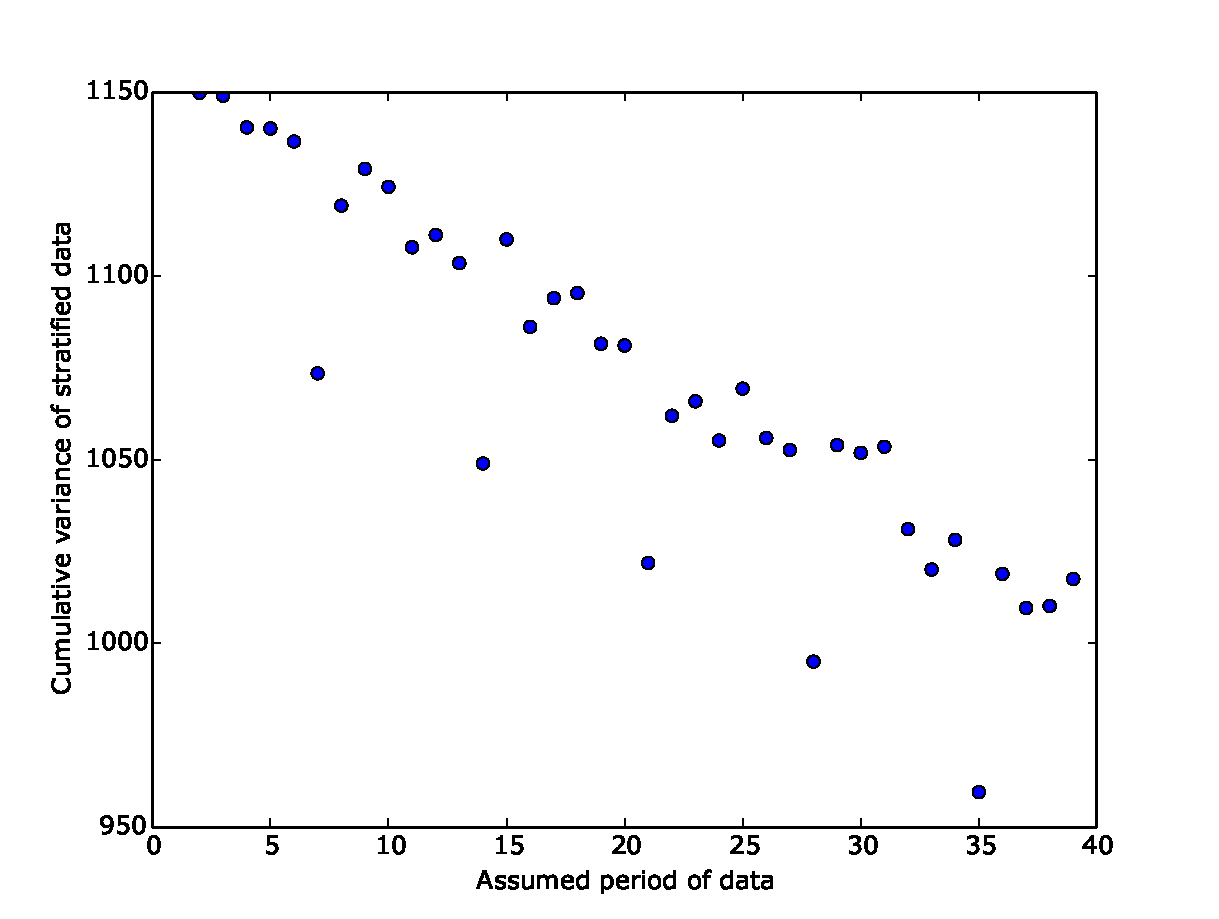
\includegraphics[scale=0.5]{Periodicity_analysis_BA_Trips.pdf}
\end{figure}

The other three links show similar dips in variance at \texttt{period} values
which are multiples of \(7\), in both data -- Travel times as well as No.\ of
Trips. \textbf{Conclusion:} NYC traffic data has a \(7\)-day periodicity.

\end{document}